\documentclass[12pt,paper=a4]{report}
\usepackage{fontspec}
\usepackage{xunicode}
\usepackage{xltxtra}
\usepackage{polyglossia}
\setdefaultlanguage{latvian}
\usepackage{fixlatvian}

\setotherlanguages{english,russian,french}
\setmainfont[Mapping=tex-text]{Times New Roman}%{LMRoman10}
% Fonts krievu valodai, kurā ir arī krievu valodas burti
\newfontfamily\russianfont{Times New Roman}
% Šos fontus tālāk izmantos chapter virsrakstos un url'os (lai būtu kirilicas burti)
\newfontfamily\sffamily{Verdana}

\usepackage{setspace}

% lai varam normāli rakstīt apakšvītras
\usepackage{underscore}
% Lai varam iekļaut attēlus
\usepackage{graphicx}
% Kurā vietā tiks meklēti attēli - relatīvais ceļs attiecībā pret dokumentu
\graphicspath{{./PNG/}{./images/internet/}{./images/self-generated/}}
% Ar šiem PDF'ā būs saliktas saites un tām va uzlikt krāsu
\usepackage{hyperref}
\hypersetup{ colorlinks, citecolor=black, filecolor=black,linkcolor=black,urlcolor=black }

\usepackage{amsmath}
\usepackage{amsfonts}
\usepackage{lipsum} %Lai ģenerētu nejaušus tekstus...
\usepackage{listingsutf8}
\usepackage{xcolor}

%\usepackage{inconsolata}
\lstset{
    language=bash, %% Troque para PHP, C, Java, etc... bash é o padrão
    basicstyle=\ttfamily\small,
    numberstyle=\footnotesize,
    numbers=left,
    backgroundcolor=\color{gray!10},
    frame=single,
    tabsize=2,
    rulecolor=\color{black!30},
    title=\lstname,
    escapeinside={\%*}{*)},
    breaklines=true,
    breakatwhitespace=true,
    framextopmargin=2pt,
    framexbottommargin=2pt,
    extendedchars=false,
    inputencoding=utf8
}


%% Mainīt chapteru izskatu - centrēts un definētais sffamily fonts (skatīt augstāk)
\usepackage{titlesec}
\titleformat{\chapter}{\huge\centering\sffamily}{\thechapter}{1pc}{}

%% Pārdēvējam ``Literatūra`` par ``Izmantotās literatūras un avotu saraksts''.
\addto\captionslatvian{
\renewcommand\bibname{Izmantotās literatūras un avotu saraksts}
}

%% Atraitņrindiņas un bāreņrindiņas ( widow orphan) vadība
\clubpenalty10000
\widowpenalty10000

%% Visādas atkāpes - 1" (2.54 cm) atkāpe jau ir pēc noklusējuma, šeit tikai korekcijas
%\setlength{\parskip}{1line}
\setlength{\topmargin}{0cm}
\setlength{\headheight}{0in}
\setlength{\headsep}{0in}
\setlength{\textheight}{22.7cm}
\setlength{\textwidth}{15cm}
\setlength{\oddsidemargin}{0.5in}
\setlength{\evensidemargin}{0.5in}
%\setlength{\parindent}{0.25in}
%\setlength{\parskip}{0.25in}

%% uzliekam atkāpes arī nodaļu 1. rindkopas 1. rindai
\usepackage{indentfirst}

%Pārnesumiem - ļauj tiasīt lielākas starpas
\hyphenpenalty=5000

%% Nodaļu un apakšnodaļu numerācija tagad to veic fixlatvian package
%\def\thechapter      {\arabic{chapter}.}
%\def\thesection      {\ifx\chapter\undefined{\arabic{section}.}\else  %{\thechapter\arabic{section}.}\fi}
%\def\thesubsection   {\thesection\arabic{subsection}.}
%\def\thesubsubsection{\thesubsection\arabic{subsubsection}.}
%\def\theparagraph    {\thesubsubsection\arabic{paragraph}.}
%\def\thesubparagraph {\theparagraph\arabic{subparagraph}.}

%% Pakotne lai saliktu automātisku figūru skaitīšanu
\usepackage{totcount}

\newcounter{nofappendices}
\setcounter{nofappendices}{0}
\regtotcounter{nofappendices}

\newtotcounter{fignum}
\def\oldfigure{} \let\oldfigure=\figure
\def\figure{\stepcounter{fignum}\oldfigure}

%defineejam atsauču skaitītāju
\newtotcounter{citnum}
\def\oldbibitem{} \let\oldbibitem=\bibitem
\def\bibitem{\stepcounter{citnum}\oldbibitem}

%% Attēlu numerācija
%\renewcommand{\thefigure}{\arabic{chapter}.\arabic{figure}.}

%% Sarakstam visus mainīgos
%% Mainīgie titullapai, defAutors tiek izmantots arī galvojumā
\def\defAutors{Edgars Skore}
\def\defAugstskola{Ventspils Augstskola}{\fontfamily{russianfont}
\def\defFakultate{Informācijas tehnoloģiju fakultāte}
\def\defSProgrammas{dabas zinātņu maģistra studiju programmas\\
	      datorzinātnēs}
\def\defStudents{2. kursa students \\
	      \defAutors}
\def\defMatrikulasNr{16080002}
\def\defDarbaNosaukums{Cilvēku plūsmas analīze, pielietojot konvolūcijas tīklus}
\def\defDarbaNosaukumsEN{Human flow analysis using Convolutional Neural Networks}
\def\defDarbaNosaukumsFR{La grande question sur la vie, l'univers et le reste}
\def\defDarbaNosaukumsLV{Pagātnes, tagadnes un nākotnes aspekti atbildei uz galveno jautājumu}
\def\defDarbaNosaukumsRU{Ответ на главный вопрос жизни, вселенной и всего такого}
\def\defDarbaVeids{Maģistra darbs}
\def\defFakultatesDekans{doc.  Dr.phys. M.~Ēlerts}
\def\defZinVaditajs{Dr.sc.comp. Gundars Bergmanis-Korāts}
\def\defGads{2018}
 %šeit pārdefinējam savus mainīgos (atstāju iepriekšējās rindas, lai varētu redzēt pārdefinēšanu)

%% pievienota anotācijas noformēšana
%\usepackage{etoolbox}% http://ctan.org/pkg/etoolbox
%\makeatletter
%\patchcmd{\@makechapterhead}{\vspace*{50\p@}}{}{}{}% Removes space above \chapter head
%\setafterchapterskip{1sp}
%defineejam anotaacijas lapas, lai vareetu vienkaarshaak taas izmantot
\def\abstract{
  %\section*{\begin{center} \abstractname \end{center}} % start chapter

\vspace*{-4\baselineskip}
	\chapter*{\begin{center} \abstractname \end{center} } % start chapter
	\vspace*{-2.5\baselineskip}
  \addcontentsline{toc}{chapter}{\abstractname} % table of contents line
  \markboth{\MakeUppercase{\abstractname}}{} % header mark
}
\def\endabstract{}%\clearpage

%% Beidzot sākam rakstīt dokumentu
\begin{document}

%% Vislabāk nodaļas rakstīt kā atseviškus failus, kurus iekļauj ar input (.tex paplašinājums pats tiek pielikts klāt)
% \input{src/mag-titullapa} %% visu titullapu ērtāk ir turēt datnē mag-titullapa.tex, bet te mēs tomēr visu rakstīsim vienā vietā:

%%%% Titullapas sākums
%%%% Titullapas sākums
\begin{titlepage}
\begin{center}
\textsc{
\defAugstskola\\
\defFakultate}\\
\vspace{2em}
\textbf{\defDarbaVeids}\\
\vspace{2em}
{\LARGE \textbf{\defDarbaNosaukums}}\\
\vspace{2em}
\begin{tabular}{@{}r@{}l@{}}
\parbox[c]{0.4\textwidth}{Autors:}&
\parbox[t]{0.6\textwidth}{
\defAugstskola s\\
\defFakultate s\\
\defSProgrammas\\
\defStudents \\
Matrikulas~Nr. \defMatrikulasNr\vspace{0.7em}\\
\mbox{}\hrulefill\vspace{-0.4em}\\
{\scriptsize(paraksts)}\vspace{2em}} \\
\parbox[c]{0.4\textwidth}{Fakultātes dekāns:}&
\parbox[t]{0.6\textwidth}{
\defFakultatesDekans\vspace{.7em}\\
\mbox{}\hrulefill\vspace{-0.4em}\\
{\scriptsize(paraksts)}\vspace{2em}} \\
\parbox[c]{0.4\textwidth}{Zinātniskais vadītājs:}&
\parbox[t]{0.6\textwidth}{
\defZinVaditajs\vspace{.7em}\\
\mbox{}\hrulefill\vspace{-0.4em}\\
{\scriptsize(paraksts)}\vspace{2em}} \\
\parbox[c]{0.4\textwidth}{Recenzents:} & \vspace{.7em}\\
\multicolumn{2}{@{}c@{}}{
\mbox{}\hrulefill
}\vspace{-0.4em}\\
\multicolumn{2}{@{}l@{}}{
{\scriptsize(Ieņemamais amats, zinātn. nosaukums,
vārds, uzvārds)}
}\vspace{.7em}\\
&\mbox{}\hrulefill\vspace{-0.4em}\\
&{\scriptsize(paraksts)}\\
\end{tabular}
\vfill
Ventspils, \defGads
\end{center}
\end{titlepage} %pievienota titullapa, kura izveidota atsevišķā failā
%%%% Titullapas beigas

%%%% Satura rādītājs
\tableofcontents

%%%% 1.5 līiniju atstarpe starp rindām
\onehalfspace

{
	\selectlanguage{latvian}
	\begin{abstract}
		
		\begin{tabular}{@{}r@{}l@{}}
			\parbox[c]{0.3\textwidth}{\textbf{The title:}}&
			\parbox[t]{0.65\textwidth}{\defDarbaNosaukumsEN} \\
			\parbox[c]{0.3\textwidth}{\textbf{Autors:}}&
			\parbox[t]{0.65\textwidth}{\defAutors} \\
			\parbox[c]{0.3\textwidth}{\textbf{Academic Advisor:}}&
			\parbox[t]{0.65\textwidth}{\defZinVaditajs} \\
			\parbox[c]{0.3\textwidth}{\textbf{The volume of the work:}}&
			\parbox[t]{0.65\textwidth}{\textcolor{black}{\pageref{LastPage}} pages, XX~tables,  \total{fignum}~images, XX~equations, \total{citnum}~literature sources, \total{nofappendices}~appendices} \\
			\parbox[c]{0.3\textwidth}{\textbf{Keywords:}}&
			\parbox[t]{0.65\textwidth}{ Life, Universe, Questions, Philosophy} \\
			&\\
		\end{tabular}
		%\total{nofimages} % ja nu gadiijumaa vajag custom counter
		
		In the first novel and radio series, a group of hyper-intelligent pan-dimensional beings demand to learn the \textbf{Answer to the Ultimate Question of Life} from the supercomputer, Deep Thought, specially built for this purpose. It takes Deep Thought 7½ million years to compute and check the answer, which turns out to be\textbf{ 42}.  Unfortunately, The Ultimate Question itself is unknown.\cite{wiki-en}
		
	\end{abstract}
}

%%%% 1.5 līiniju atstarpe starp rindām
\onehalfspace
{
\selectlanguage{english}
\begin{abstract}

\begin{tabular}{@{}r@{}l@{}}
\parbox[c]{0.3\textwidth}{\textbf{The title:}}&
\parbox[t]{0.65\textwidth}{\defDarbaNosaukumsEN} \\
\parbox[c]{0.3\textwidth}{\textbf{Author:}}&
\parbox[t]{0.65\textwidth}{\defAutors} \\
\parbox[c]{0.3\textwidth}{\textbf{Academic Advisor:}}&
\parbox[t]{0.65\textwidth}{\defZinVaditajs} \\
\parbox[c]{0.3\textwidth}{\textbf{The volume of the work:}}&
\parbox[t]{0.65\textwidth}{\textcolor{black}{\pageref{LastPage}} pages, XX~tables,  \total{fignum}~images, XX~equations, \total{citnum}~literature sources, \total{nofappendices}~appendices} \\
\parbox[c]{0.3\textwidth}{\textbf{Keywords:}}&
\parbox[t]{0.65\textwidth}{ Life, Universe, Questions, Philosophy} \\
&\\
\end{tabular}
%\total{nofimages} % ja nu gadiijumaa vajag custom counter

In the first novel and radio series, a group of hyper-intelligent pan-dimensional beings demand to learn the \textbf{Answer to the Ultimate Question of Life} from the supercomputer, Deep Thought, specially built for this purpose. It takes Deep Thought 7½ million years to compute and check the answer, which turns out to be\textbf{ 42}.  Unfortunately, The Ultimate Question itself is unknown.\cite{wiki-en}

\end{abstract}
}

%%%% Nodaļa bez numerācijas
\chapter*{Izmantotie saīsinājumi un termini}
\addcontentsline{toc}{chapter}{Izmantotie saīsinājumi un termini}

%%%  Sākas nodaļas
\chapter{Ievads}
Ievadā ir jāietver:

\begin{itemize}
\item temata aktualitātes pamatojums;
\item darba mērķis;
\item darba mērķa sasniegšanai veicamo uzdevumu formulējums;
\item izmantojamo pētīšanas metožu un paņēmienu uzskaitījums;
\item literatūras un avotu grupu uzskaitījums (piemēram, speciālā ekonomiskā literatūra, valsts statistikas dati, nepublicētie materiāli no uzņēmuma arhīva u.c.);
\item darba struktūras apraksts;
\item pētījuma temata un perioda norobežojums (ja tas nepieciešams).
\end{itemize}

Mašīnmācīšanās algoritmi ir kļuvuši par neatņemamu sastāvdaļu programmatūras izstrādātājiem un kompānijām, kas savas aplikācijas grib padarīt "gudras". Lai arī cik, mūsdienās, šis jēdziens ir kļuvis populārs, oficiāla mašīnmācīšanās definīcija nav noteikta. Visvienkāršākais mašīnmācīšanās pielietojums ir apstrādāt datus, mācīties no tiem un no iegūtajiem rezultātiem pieņemt lēmumus vai veikt minējumus reālās pasaules problēmu risināšanai. Tā vietā, lai manuāli veidotu programmatūras risinājumus, kas veic kādu uzdevumu, tiek apmācīti datori vai citas ierīces, izmantojot lielus datu apjomus. 
\section{Mašīnmācīšanās pamatjēdziens}
Pasaulē ir daudz un dažādi mašīnmācīšanās algoritmi un katru dienu tiek publicēti simtiem jaunu algoritmu. Tos var sagrupēt pēc apmācības veida (vadītā apmācība (\textit{supervised learning}), nevadītā apmācība (\textit{unsupervised learning}), pusvadītā apmācība (\textit{semi-supervised learning})) kā arī pēc formas vai funkcijas līdzībām (klasifikācija, regresija, lēmumu koki (\textit{decision trees}), klasterēšana (\textit{clustering}), dziļā mašīnmācīšanās (\textit{deep learning})). Neatkarīgi no apmācības veida vai pielietojuma, visas mašīnmācīšanās algoritmu kombinācijas sastāv no klasifikatoriem (atbalsta vektora mašīna, lēmuma koki, neironu tīkli), vērtēšanas funkcijām (varbūtības funkcijas, robežfunkcijas, izmaksu funkcija) un optimizācijas funkcijām (mantkārīgā meklēšana, nepārtrauktās optimizācijas metodes (\textit{continuous optimization})). Izmantojot šīs sastāvdaļas, mašīnmācīšanās algoritmu pamata mērķis ir būt spējīgam funkcionēt ne tikai ar apmācībā piedāvātajiem datiem, bet arī spēt darboties ar datiem, ar kuriem algoritms nav saskāries. Atkarībā no veicamā uzdevuma, ir dažādi veidi kā panākt, lai datori vai jebkura cita ierīce mācās, sākot ar visparastākajiem lēmumu kokiem, beidzot ar ģenētiskajiem algoritmiem un mākslīgajiem neironu tīkliem. 


\newpage
\section{Datorredze}
Datorredze (no angļu val. \textit{computer vision}) ir datorzinātņu nozare, kuras mērķis ir ļaut datoriem redzēt un veikt tādus pašus uzdevumus kā cilvēki veiktu ar acīm un darīt to tikpat efektīvi. Redzes nodrošināšana datoriem nozīmē dot tiem spēju identificēt un apstrādāt attēlus līdzīgi kā to spēj darīt cilvēki. Tas ir kā nodot cilvēku inteliģenci un instinktus datoram. Datorredzes sistēmas parasti iedala trīs komponentēs:
\begin{itemize}
	\item Attēla iegūšana;
	\item Attēla apstrāde;
	\item Attēla analīze;
\end{itemize}
Līdzīgi kā cilvēku pasaules izpratne balstās uz spēju pieņemt lēmumus ņemot vērā redzēto, piedāvājot datoriem šādu vizuālu izpratni, tiem būtu iespējams pieņemt patstāvīgus lēmumus.

\begin{figure}[h]%
	\centering
	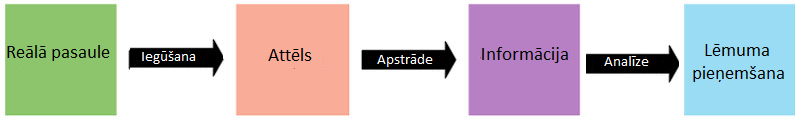
\includegraphics[height=2cm]{images/computervision1.png} %
	\caption{Datorredzes pamatprincips}%
	\label{fig:example}%
\end{figure}

Attēlu iegūšana ir process kurā reālās pasaules notikumi tiek pārveidoti bināros datos, kurus interpretē kā digitālus attēlus vai kā daļu no video fragmenta. 

Attēlu apstrāde ir iegūto attēlu zema līmeņa apstrāde. Pirmajā solī iegūtajiem binārajiem datiem pielieto algoritmus, kas norāda uz attēla daļām, kas satur zema līmeņa informāciju. Šādu informāciju var izšķirt pēc jebkādiem ģeometriskiem elementiem, kas sastāda attēlu, piemēram, punkti attēlā, attēla malas vai segmenti. Zema līmeņa attēlu apstrādes algoritmi ir malu detektēšana, segmentācijas algoritmi, klasifikācija, īpašību detektēšana.
\begin{figure}[h]%
	\centering
	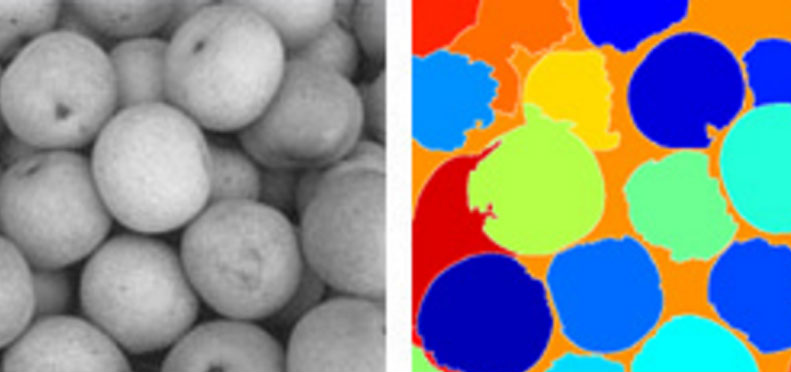
\includegraphics[height=3cm]{images/computervision2.png} %
	\caption{Ābolu segmentācija attēlā \cite{compv1}}%
	\label{fig:example}%
\end{figure} 

Pēdējā datorredzes sistēmu komponente ir attēlu analīzes solis, kurā notiks attēla analīze un pēc šī soļa datorredzes sistēmai būs iespējams pieņemt lēmumu un izvadē to atgriezt. Attēlu analīzes solī tiek pielietoti augsta līmeņa algoritmi, ņemot vērā gan attēla apstrādes solī iegūto zema līmeņa informāciju, gan pašu attēlu. Piemēri kur var izmantot šādu augsta līmeņa attēlu analīzi ir trīsdimensiju ainu atveidošana, objektu atpazīšana, objektu sekošana, cilvēku plūsmas analīze.
\begin{figure}[h]%
	\centering
	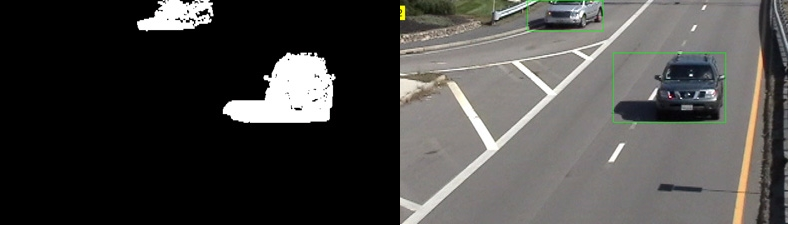
\includegraphics[height=4cm]{images/computervision3.png} %
	\caption{Objektu detektēšana pēc segmentācijas pielietošanas \cite{compv2}}%
	\label{fig:example}%
\end{figure} 

Izstrādājot datorredzes sistēmas, pētnieki saskaras ar dažādām problēmām un izaicinājumiem. Parasti šīs problēmas ir atkarīgas no datu kvalitātes, sistēmas pielietojuma un apkārtējās pasaules ietekmes uz datiem un aparatūru. Datorredzes pētnieki izstrādā risinājumus, lai padarītu datorredzes algoritmus stabilākus un efektīvākus sarežģītos uzstādījumos: nekvalitatīvi vai trokšņaini dati, reālā laika apstrāde un ierobežota skaitļošanas jauda. Mūsdienās, lai risinātu šīs problēmas, tiek savienoti mašīnmācīšanās risinājumi ar datorredzes risinājumiem.

Klasiskie datorredzes algoritmi ir smalki pētīti un optimizēti, lai iegūtu labāko veiktspēju un lai tie efektīvi izmantotu datora skaitļošanas resursus, kamēr mašīnmācīšanās algoritmi piedāvā precīzākus un vispusīgākus risinājumus, taču prasa lielus skaitļošanas resursus. Ņemot vērā iepriekš minēto, mūsdienu pētījumos ir populāri risinājumi, kas apvieno standarta datorredzes algoritmus un mašīnmācīšanās risinājumus. Labs piemērs abu šo nozaru apvienošanā ir kustīgu objektu meklēšana video fragmentos. Lai iegūtu augstāku precizitāti un taupītu skaitļošanas resursus ir iespējams attēla apstrādi veikt ar datorredzes algoritmiem un attēla analīzi (klasifikāciju, lokalizāciju, sekošanu) veikt ar neironu tīkliem.



 %% Ērtāk visu ir rakstīt atsevišķos failos - ievads.tex un tad tos iekļaut ar input komandu

\chapter{Mašīnmācīšanās}
Mašīnmācīšanās algoritmi ir kļuvuši par neatņemamu sastāvdaļu programmatūras izstrādātājiem un kompānijām, kas savas aplikācijas grib padarīt "gudras". Lai arī cik, mūsdienās, šis jēdziens ir kļuvis populārs, oficiāla mašīnmācīšanās definīcija nav noteikta. Visvienkāršākais mašīnmācīšanās pielietojums ir apstrādāt datus, mācīties no tiem un no iegūtajiem rezultātiem pieņemt lēmumus vai veikt minējumus reālās pasaules problēmu risināšanai. Tā vietā, lai manuāli veidotu programmatūras risinājumus, kas veic kādu uzdevumu, tiek apmācīti datori vai citas ierīces, izmantojot lielus datu apjomus. 
\section{Pamatjēdziens}
Pasaulē ir daudz un dažādi mašīnmācīšanās algoritmi un katru dienu tiek publicēti simtiem jaunu algoritmu. Tos var sagrupēt pēc apmācības veida (vadītā apmācība (\textit{supervised learning}), nevadītā apmācība (\textit{unsupervised learning}), pusvadītā apmācība (\textit{semi-supervised learning})) kā arī pēc formas vai funkcijas līdzībām (klasifikācija, regresija, lēmumu koki (\textit{decision trees}), klasterēšana (\textit{clustering}), dziļā mašīnmācīšanās (\textit{deep learning})). Neatkarīgi no apmācības veida vai pielietojuma, visas mašīnmācīšanās algoritmu kombinācijas sastāv no klasifikatoriem (atbalsta vektora mašīna, lēmuma koki, neironu tīkli), vērtēšanas funkcijām (varbūtības funkcijas, robežfunkcijas, izmaksu funkcija) un optimizācijas funkcijām (mantkārīgā meklēšana, nepārtrauktās optimizācijas metodes (\textit{continuous optimization})). Izmantojot šīs sastāvdaļas, mašīnmācīšanās algoritmu pamata mērķis ir būt spējīgam funkcionēt ne tikai ar apmācībā piedāvātajiem datiem, bet arī spēt darboties ar datiem, ar kuriem algoritms nav saskāries. 

Atkarībā no veicamā uzdevuma, ir dažādi veidi kā panākt, lai datori vai jebkura cita ierīce mācās, sākot ar visparastākajiem lēmumu kokiem, beidzot ar ģenētiskajiem algoritmiem un mākslīgajiem neironu tīkliem. Lēmumu koki atspoguļo reālās dzīves koka struktūru un tos izmanto gan klasifikācijas, gan regresijas problēmu risināšanā. Analizējot datus, lēmumu kokus var izmantot, lai vizuāli aprakstītu lēmumus un lēmumu pieņemšanu. Mašīnmācīšanās gadījumā, lēmumu kokus apraksta kā klasifikācijas kokus vai regresijas kokus (\textit{CART - Classification and Regression Trees}), atkarībā no veicamā uzdevuma. Galvenā šo koku doma ir audzēt zarus, pieņemot lēmumus, kuras koka īpašības izvēlēties, zinot apstāšanās nosacījumu. \cite{dectree}

Ģenētiskie algoritmi ir vēl viens algoritmu veids, kuru ir vērts izcelt. Tie ir algoritmi, kuri tiek izveidoti, balstoties uz notikumiem, kurus novēro dabīgajos evolūcijas procesos. Datorzinātnē ģenētiskie algoritmi ir optimizācijas algoritmi, kuri prot patstāvīgi apgūt jaunu informāciju, balstoties uz evolūcijas jēdzieniem kā dabīgā atlase un ģenētika. Ģenētisko algoritmu pamatideja ir simulēt Čārlza Dārvina piedāvāto teorēmu "izdzīvo stiprākais". Risinot problēmu, ģenētiskais algoritms saglabā tikai spēcīgākos indivīdus katrā paaudzē. Šie indivīdi sacenšas par resursiem un iespēju veidot nākamo paaudzi. Jaunās paaudzes tiek veidotas izvēloties vecākus no iepriekšējās paaudzes, veicot \textit{crossover} operāciju un mutāciju. Spēcīgākie indivīdi katrā paaudzē izveidos vairāk pēcnācēju nekā vājie indivīdi, tādējādi katra nākamā indivīdu paaudze kļūs labāka, galu galā iegūstot labāko rezultātu problēmas risināšanai. Beigu nosacījumu nosaka pirms algoritma izpildes, parasti, tiek noteikts paaudžu skaits vai kāds labāko indivīdu rezultātu slieksnis, kuru pēcnācēju paaudze pārsniedz. Ģenētiskie algoritmi gan nespēj risināt klasifikācijas problēmas, bet tos lieto kā optimizācijas funkciju. Lai rēķinātu neironu tīklu svarus, var izmantot ģenētiskos algoritmus. \cite{genalg}
\begin{figure}[h]%
	\centering
	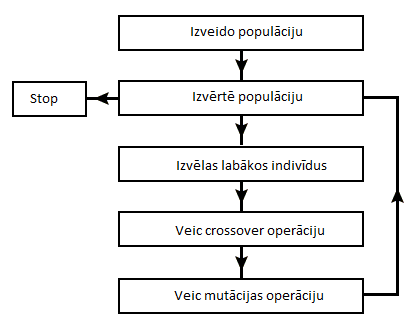
\includegraphics[height=6cm]{images/gen-algo-bilde.png} %
	\caption{Ģenētisko algoritmu modelis}%
	\label{fig:example}%
\end{figure}

Mākslīgie neironu tīkli ir viena no populārākajām mašīnmācīšanās izmantotajām metodēm. Tas ir neapstrādāts elektronisks modelis, kas balstīts uz smadzeņu bioloģisko neironu tīklu. Var teikt, ka šāda neironu tīkla modelis, līdzīgi kā smadzenes, mācās no pieredzes. Teorētiski, šādu smadzeņu modelēšana, paredz, ka šāds mašīnmācīšanās risinājums, neprasa dziļas tehniskas zināšanas bioloģijā vai datorzinātnē, bet ir jāspēj tīklu izveidot pareizi kopā saliekot vairākas slāņu kārtas. Šādas, bioloģijas iedvesmotas metodes uzskata par nākamo lielo soli datorzinātnes industrijā.\cite{staff} \par
Iedziļinoties mākslīgo neironu tīklu uzbūvē, neironu tīkls sastāv no daudz, savstarpēji savienotiem mezgliem, kur katrs no mezgliem veic kādu matemātisku operāciju. To, ko atgriež katrs mezgls, nosaka matemātiskā operācija, ko šis mezgls veic kā arī citi parametri, kas specifiski šim mezglam. Šie mezgli galu galā tiek grupēti un šos mezglu grupējumus sauc par slāņiem (no ang. val. - \textit{layer}). \par
Mākslīgie neironu tīkli satur sava veida "mācīšanās likumus", kas ir process, kad tiek mainīti mezglu savienojumu svari atkarībā no informācijas ievadē. 
Kad neironu tīkls ir apmācīts tik tālu, ka lietotājs ir apmierināts, tad tīklam var sākt piedāvāt datus, kuri tad iziet cauri visiem slāņiem, tādā veidā turpinot mācības uz sākumā izveidotā modeļa bāzes. Neironu tīklus ir arī iespējams pārtrenēt, kas nozīmē, ka tīkls atpazīst tikai vienu ienākošo datu tipu. Ja tā notiek, tad mācīšanās vairs nav iespējama. Mākslīgos neironu tīklus izmanto dažādu problēmu risināšanai, dažādās apakšnozarēs un šī darba nolūkos autors neironu tīklus izmantos dziļajai apmācībai.
\begin{figure}[h]%
	\centering
	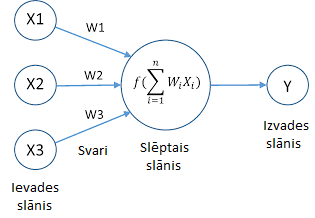
\includegraphics[height=5cm]{images/neironutikls.png} %
	\caption{Vienkāršs neironu tīkla modelis}%
	\label{fig:example}%
\end{figure}
\section{Dziļā mašīnmācīšanās}
Mašīnmācīšanās no dziļās mašīnmācīšanās atšķiras ar to, ka mašīnmācīšanās ir sarežģīti izmantot ļoti lielas datu kopas, taču ar dziļās apmācības metodēm tas ir iespējams. Dziļās mašīnmācīšanās metodes atgriež jebkādas vērtības sākot ar skaitliskām vērtībām, beidzot ar elementiem kā attēli, teksts vai skaņa, taču parastās mašīnmācīšanās metodes spēj atgriezt tikai skaitliskas vērtības kā, piemēram, klasifikācijas indeksu vai kādas funkcijas rezultātu. Mašīnmācīšanās izmanto dažādus automatizētus algoritmus, kas iemācās modeļa funkcijas un paredz nākotnes darbības no padotajiem datiem, kamēr dziļā apmācībā izmanto neironu tīklus, kas laiž datus caur daudz apstrādes slāņiem, lai izšķirtu datu īpašības. Lielākā atšķirība, pēc autora domām, starp mašīnmācīšanos un dziļo mašīnmācīšanos ir tajā, ka dziļās mašīnmācīšanās metodes automātiski datos atrod svarīgās īpašības, kamēr mašīnmācīšanās algoritmos šīs īpašības ir manuāli jānorāda. 
\begin{figure}[h]%
	\centering
	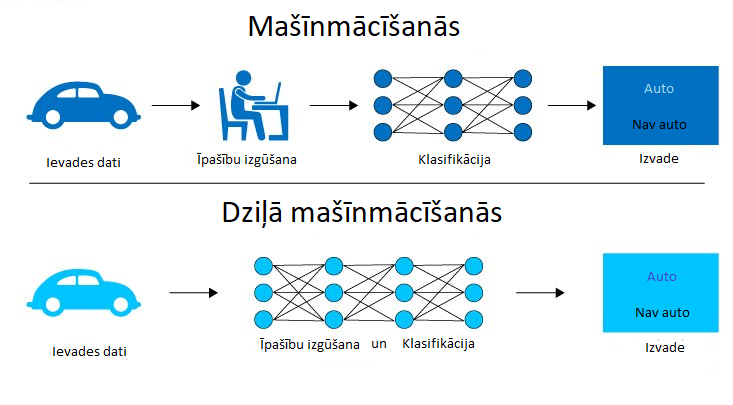
\includegraphics[height=7cm]{images/deeplearning.png} %
	\caption{Mašīnmācīšanās un dziļās mašīnmācīšanās salīdzinājums}%
	\label{fig:example}%
\end{figure}
Dziļā mašīnmācīšanās ļauj apmācīt matemātiskus modeļus, kas izveidoti no vairākiem datu apstrādes slāņiem, ar datiem, kas attēloti kā vairāku līmeņu abstrakcija (pētamā objekta galveno īpašību izdalīšana un mazsvarīgu aspektu ignorēšana). Šīs metodes ir uzlabojušas jaunākās tehnoloģijas balss atpazīšanā, objektu atpazīšanā attēlos, objektu detektēšanā. Dziļā mašīnmācīšanās, izmantojot atpakaļdatošanas algoritmus, sarežģītās datu kopu struktūrās meklē kā datoram vai jebkurai citai ierīcei būtu jāmaina iekšējie parametri starp tīklu slāņiem.

Īpašību apmācība ir metožu kopums, kas atļauj ierīcei padot neapstrādātus datus un automātiski iegūt īpašības, kas nepieciešamas, lai veiktu detektēšanu vai klasifikāciju. Dziļās mašīnmācīšanās metodes ir īpašību apmācības metodes ar vairākiem īpašību slāņiem, kurus iegūst apvienojot vienkāršus, taču nelineārus modeļus, kur katrs modelis pārveido īpašību no viena līmeņa uz augstāku, abstraktāku līmeni. Veicot pietiekami daudz šādus pārveidojumus, algoritmiem ir iespējams iemācīties ļoti sarežģītas darbības.\cite{deepnet} Darba ietvaros, objektu detektēšanai tiks izmantots konvolūciju neironu tīkls (\textit{CNN}), kas ir dziļās mašīnmācīšanās tips.

\section{Konvolūcijas neironu tīkli}
Konvolūcijas neironu tīkli (turpmāk \textit{CNN}) ir izveidoti, lai apstrādātu datus, kas ievadei padoti kā vairāki masīvi, piemēram, divdimensiju masīvi, kas satur pikseļu intensitātes vairākos krāsu kanālos (attēls). Vairākus datu veidus vienkāršojot, tos var izteikt kā masīvus: viendimensijas masīvs priekš signāliem vai skaitļu rindām, divdimensiju masīvi attēliem vai audio spektogrammām un trīsdimensiju masīvs video. Vislabāko rezultātu CNN tīklu veidi sasniedz risinot objektu detektēšanas, segmentācijas vai klasifikācijas problēmas.

Līdzīgi parastajiem neironu tīkliem arī konvolūciju neironu tīkli ir izveidoti no vairākiem slāņiem.

\subsection{Tīklu slāņi}
\subsubsection{title1}
\subsubsection{title2}
\subsubsection{title3}
\subsubsection{title4}
\subsection{Tīklu arhitektūras}
\subsubsection{title1}
\subsubsection{title2}
\subsubsection{title11}
\subsubsection{title22}
\subsection{Tīklu apmācība}

\chapter{Detektēšana un sekošana}
aprakstīt kapēc detektēt un trackot, kapēc nevar tikai detektēt
\section{Detektēšana}
\subsection{SSD}
\subsection{YOLO}
\subsection{Faster R-CNN}
\section{Sekošana}
\subsection{AdaBoost}
\subsection{Multiple Instance Learning}
\subsection{Kernelized Correlation Filters}
\subsection{SiamFC}
\chapter{Implementācija}
\section{Datu sagatavošana}
\section{Detektēšana}
\subsection{caffe}
\subsubsection{Tīklu apmācība}
\subsubsection{Detektēšana}
\paragraph{SSD}
\paragraph{Faster R-CNN}
\subsection{darknet}
\subsubsection{Tīklu apmācība}
\subsubsection{Detektēšana izmantojot YOLO}
\section{Sekošana}
\subsection{OpenCV sekošanas programmējamā saskarne (API)}
\subsection{SiamFC}
%% Nenumurēta nodaļa, kas uzrādās satura rādītājā
\chapter*{Secinājumi un priekšlikumi}
\addcontentsline{toc}{chapter}{Secinājumi un priekšlikumi}
\begin{enumerate}
\item \textbf{Secinājumi un priekšlikumi} jāraksta tēžu veidā.
\item Secinājumiem jāatspoguļo svarīgākās atziņas, kas izriet no pētījuma, satur atbildes uz ievadā izvirzīto mērķi un uzdevumiem.
\item Secinājumos jāpaskaidro veiktā pētījuma tautsaimnieciskā, zinātniskā vai praktiskā nozīme un autora personīgais veikums uzdevuma risināšanā.
\item Secinājumus nedrīkst pamatot ar datiem un faktiem, kas nav minēti darbā.
\item Secinājumos nav pieļaujami citāti no citu autoru darbiem, tajos jāatspoguļo tikai darba autora domas, spriedumi, atziņas.
\item Priekšlikumiem jāizriet no darbā veiktajiem pētījumiem un izdarītajiem secinājumiem, tiem jābūt konkrētiem un pamatotiem.
\item Priekšlikumos apkopo arī darbā pamatotās rekomendācijas trūkumu novēršanai.
\item Secinājumi un priekšlikumi jānumurē ar arābu cipariem.
\end{enumerate}
 %% Ērtāk visu failā secinajumi-un-priesklikumi.tex

\bibliographystyle{unsrt}
\selectlanguage{latvian}
\bibliography{src/links,src/articles,src/books}	%to load the *.bib files ../articles,../books,
\addcontentsline{toc}{chapter}{Izmantotās literatūras un avotu saraksts}


\chapter*{Galvojums}
\addcontentsline{toc}{chapter}{Galvojums}
 Ar šo es, \defAutors, galvoju, ka maģistra darbs ir izpildīts patstāvīgi un bez citu palīdzības. No svešiem pirmavotiem ņemtie dati un definējumi ir uzrādīti darbā. Šis darbs tādā vai citādā veidā nav nekad iesniegts nevienai citai pārbaudījumu komisijai un nav nekur publicēts.

\vspace{1in}
\defGads.gada \rule{1cm}{0.2pt}.\rule{3cm}{0.2pt}
\label{LastPage}

%% Te vajadzētu pielikumus
\appendix
\chapter{Pirmais pielikums}

\addtocounter{nofappendices}{1}
\label{appendix:tituldati}
%\lstinputlisting[firstline=6, lastline=15]{../codes/calcHomogInfModel.m}
\lstinputlisting[firstline=18, lastline=25]{README.md}

\chapter{Otrais pielikums}

\addtocounter{nofappendices}{1}
\label{appendix:tituldati2}
\lstinputlisting{README.md}

%% Vēl jāpievieno atzīmes lapa
\pagebreak
%% Šai lapai nevajag numerāciju
\pagestyle{empty}
\begin{center}
 Maģistra darbs aizstāvēts Valsts pārbaudījumu komisijas sēdē\\
 \vspace{1em}
\end{center}
\defGads.gada \rule{1cm}{0.2pt} . \rule{3cm}{0.2pt}\\\\
un novērtēts ar atzīmi \rule{4cm}{0.2pt} \\\\\\
Protokols Nr. \rule{1cm}{0.2pt}\\\\\\
Valsts pārbaudījumu komisijas \\\\
priekšsēdētājs \rule{7cm}{0.2pt}.\\
\hspace*{5cm}\textit{\raisebox{1em}{paraksts}}


\end{document}
